%%%%%%%%%%%%%%%%%%%%%%%%%%%%%%%%%%%%%%%%%
% Medium Length Graduate Curriculum Vitae
% LaTeX Template
% Version 1.1 (9/12/12)
%
% This template has been downloaded from:
% http://www.LaTeXTemplates.com
%
% Original author:
% Rensselaer Polytechnic Institute (http://www.rpi.edu/dept/arc/training/latex/resumes/)
%
% Important note:
% This template requires the res.cls file to be in the same directory as the
% .tex file. The res.cls file provides the resume style used for structuring the
% document.
%
%%%%%%%%%%%%%%%%%%%%%%%%%%%%%%%%%%%%%%%%%

%----------------------------------------------------------------------------------------
%	PACKAGES AND OTHER DOCUMENT CONFIGURATIONS
%----------------------------------------------------------------------------------------

\documentclass[margin, 10pt]{res} % Use the res.cls style, the font size can be changed to 11pt or 12pt here

\usepackage{helvet,graphicx} % Default font is the helvetica postscript font
%\usepackage{newcent} % To change the default font to the new century schoolbook postscript font uncomment this line and comment the one above

\setlength{\textwidth}{5.1in} % Text width of the document

\begin{document}

%----------------------------------------------------------------------------------------
%	NAME AND ADDRESS SECTION
%----------------------------------------------------------------------------------------

%\begin{minipage}{0.79\textwidth}
  \moveleft.5\hoffset\centerline{\large\bf Carl Chittenden} % Your name at the top
 
  \moveleft\hoffset\vbox{\hrule width 1.2\textwidth height 1pt}\smallskip
  
  \moveleft.5\hoffset\centerline{Maycroft, Lewes Road} % Your address
  \moveleft.5\hoffset\centerline{Horsted Keynes, RH17 7DP}
  \moveleft.5\hoffset\centerline{+44 (0)7816 35 8232 --- carltc@hotmail.co.uk}
%\end{minipage}
%\begin{minipage}{0.2\textwidth}
%	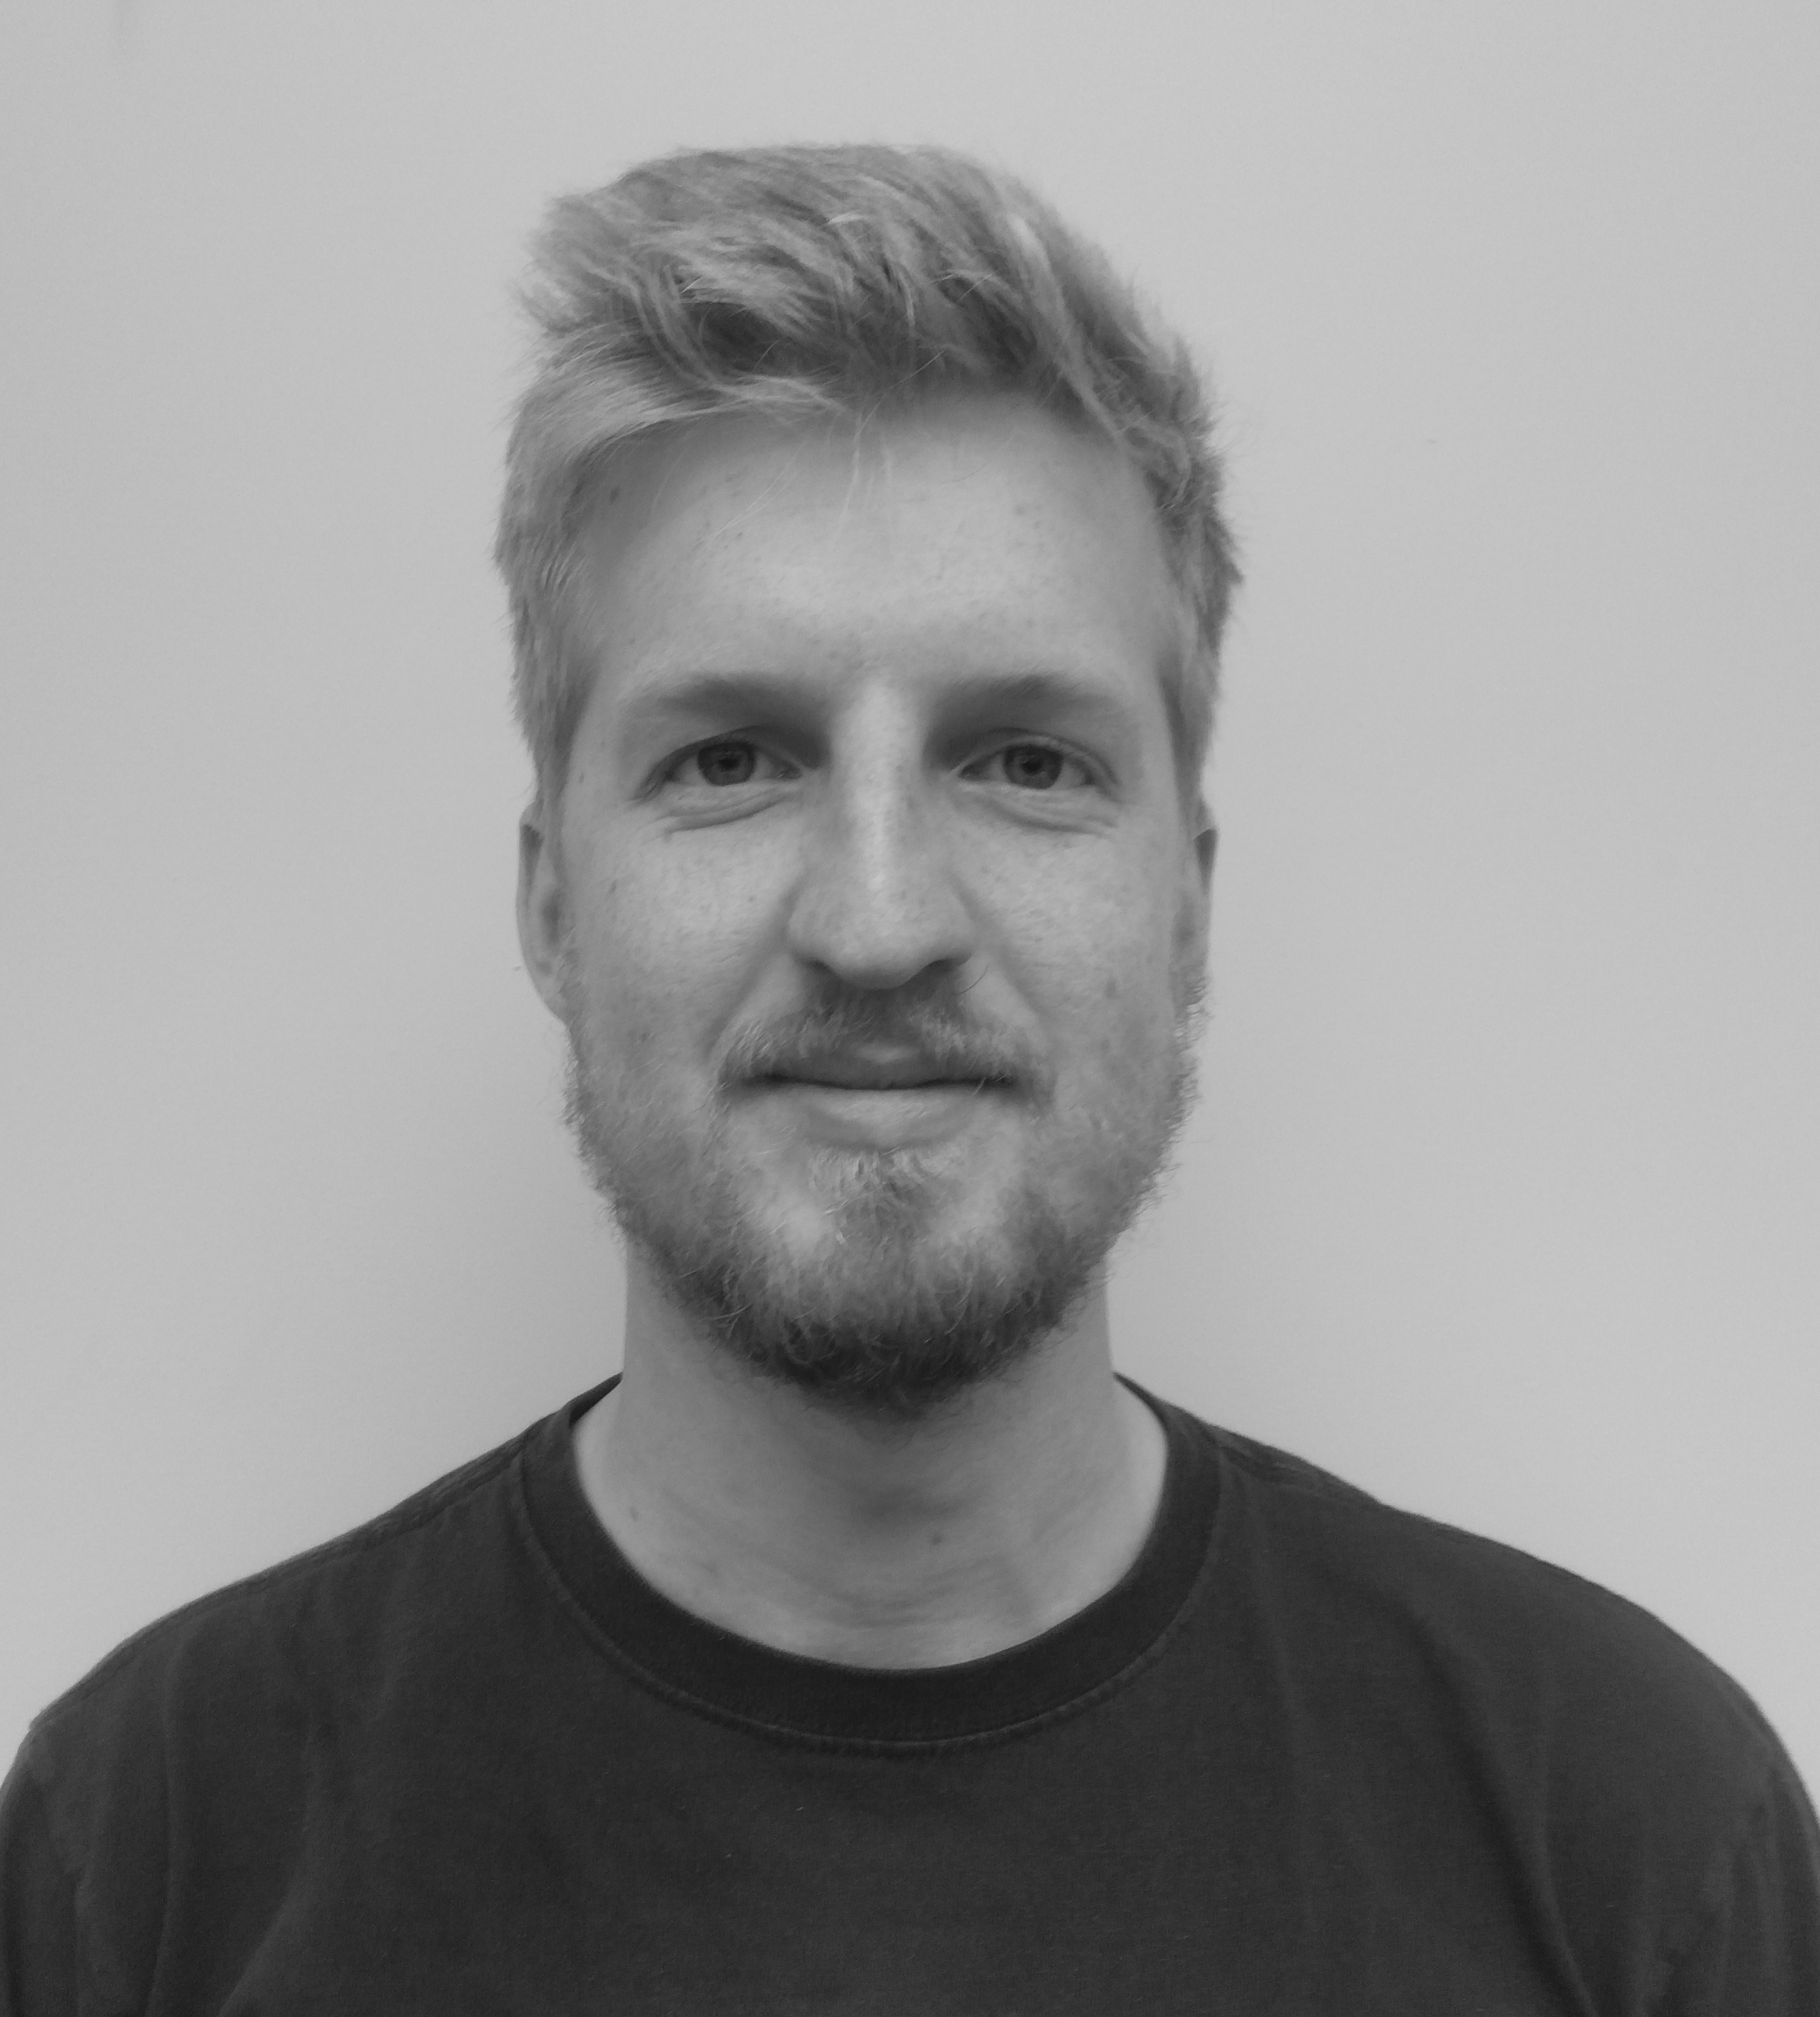
\includegraphics[width=1.4\textwidth]{image.jpg}
%\end{minipage}
%----------------------------------------------------------------------------------------

\begin{resume}
%----------------------------------------------------------------------------------------
%	OBJECTIVE SECTION
%----------------------------------------------------------------------------------------
\section{OBJECTIVE}  
Looking to start a career in video games focusing on back-end application development.
%----------------------------------------------------------------------------------------
%	EDUCATION SECTION
%----------------------------------------------------------------------------------------
%\vspace{-1cm}
\section{EDUCATION}

{\sl Ph.D.,} Electrical Engineering \\
University of Bath, Bath, UK, September 2018 \\
Thesis: Planar Array ECT for Landmine Detection

{\sl Masters,} Integrated Mechanical and Electrical Engineering \\
University of Bath, Bath, UK, September 2014 \\
Dissertation: 3D Face Recognition with Microsoft Kinect
 
%----------------------------------------------------------------------------------------
%	COMPUTER SKILLS SECTION
%----------------------------------------------------------------------------------------

\section{COMPUTER \\ SKILLS} 

{\sl Languages:} 
C\#, MATLAB, C++, Javascript, Arduino, Python, HTML/CSS, SQL Server, jQuery, VBA, WPF, Perl, Bash, LaTeX, TikZ. \\
{\sl Software:} Windows, Visual Studio, MATLAB, GitHub, Arduino, Azure, IDLE, Linux, Blender, MS Office, TeXStudio, Autodesk Inventor, Solid Edge, openGL, openCV. 
 
%----------------------------------------------------------------------------------------
%	PROFESSIONAL EXPERIENCE SECTION
%----------------------------------------------------------------------------------------
 
\section{EXPERIENCE}

{\sl Ph.D. Researcher} \hfill Sep. 2015 - Sep. 2018 \\
Department of Electronic and Electrical Engineering, University of Bath, UK
\begin{itemize} 
\item Custom PCB design and manufacture, micro-controller implementation and multi system integration for multi-channel signal switching hardware.
\item Software toolbox development for tomography system simulation and image reconstruction.
\end{itemize}

{\sl Ski Instructor} \hfill May 2015 - Sep. 2015 \\
NZSki, Mt. Hutt, NZ
\begin{itemize} 
\item Instructed skiing to various levels of ability.
\end{itemize}

{\sl IT Engineer} \hfill Sep. 2014 - May 2015 \\
Marshall-Wace Asset Management, London, UK 
\begin{itemize} 
\item Worked on C\# back-end application development for financial trading systems.
\item Managed company infrastructure on Windows and Linux.
\end{itemize} 

{\sl Design Engineer} \hfill Sep. 2011 - Sep. 2012 \\
Parker Hannifin, Watford, UK and Cologne, DE
\begin{itemize}
\item CANbus test rig design and development for hydraulic systems.
\item Marketing insight tool application programming in C\# and VB.NET.
\end{itemize} 

%----------------------------------------------------------------------------------------
%	LANGUAGES SECTION
%---------------------------------------------------------------------------------------- 

\section{LANGUAGES}

ENGLISH --- fluent/native\\
SWEDISH --- fluent/native\\
GERMAN --- conversational

%----------------------------------------------------------------------------------------
%	EXTRA-CURRICULAR ACTIVITIES SECTION
%----------------------------------------------------------------------------------------

\section{EXTRA-CURRICULAR \\ ACTIVITIES} 

Elected {\it Faculty Representative}, Electrical Engineering, Oct. 2015 - Sep. 2017 \\
Elected {\it Engagement Representative}, Postgraduate Committee, Oct. 2015 - Sep. 2018 \\
\vspace{-0.5cm}

Football {\it Starting 11}, Bath Brewhouse FC, Jun. 2016 - Sep. 2018 \\
Karate {\it 6th Kyu}, University of Bath Karate Club, Sep. 2009 - Jan. 2014

%----------------------------------------------------------------------------------------

\end{resume}
\end{document}